\section[DNA]{DNA as a information storage unit}
\label{intro-sec:DNA}

\begin{figure}[!ht]
\centering
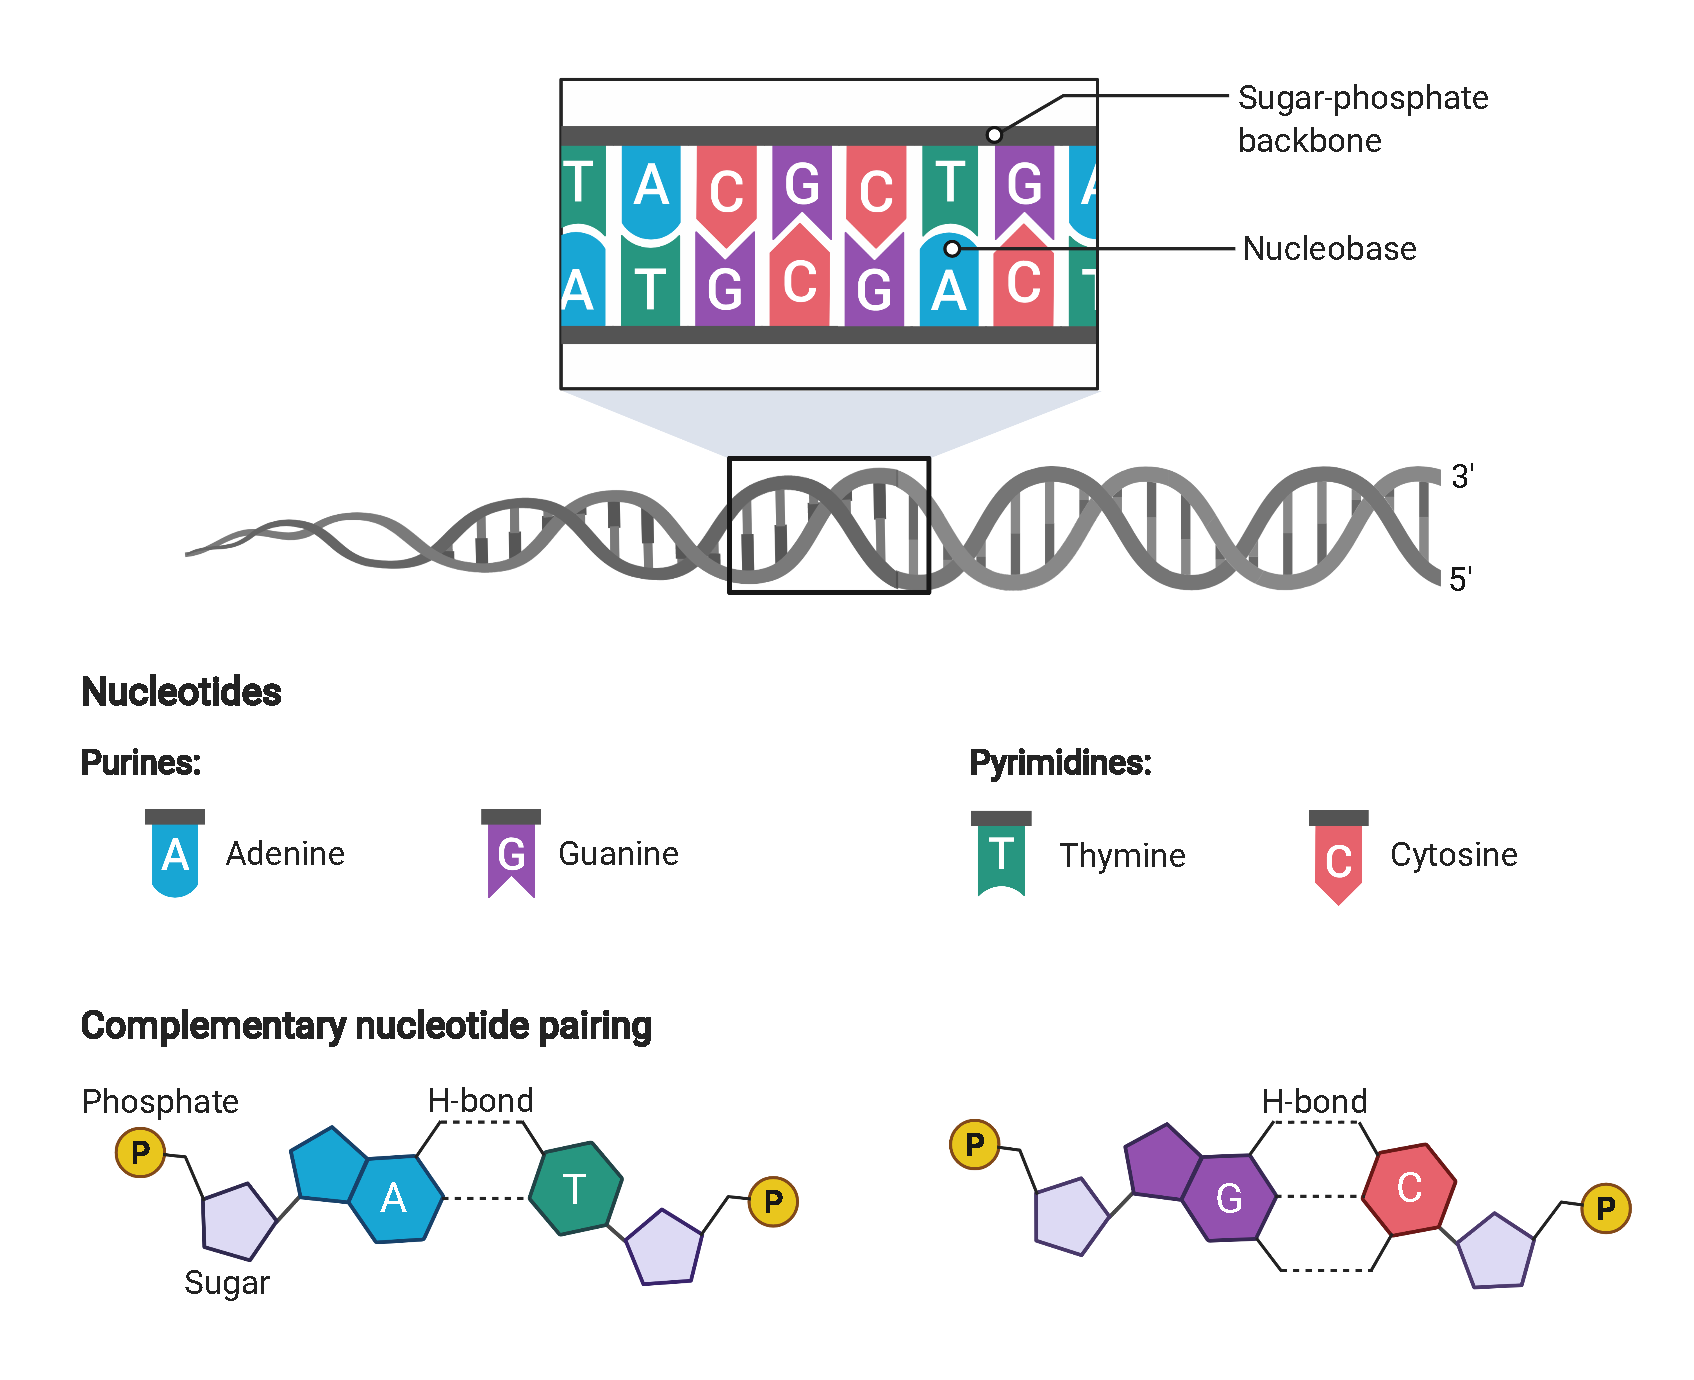
\includegraphics[width=0.9\linewidth]{Figures/DNAStructure}
\caption[Overview DNA structure]{Overview of DNA structure and the nucleobases, which form DNA strands. Nucleotides are split into Purines and Pyrimidines by the structure of the nitrogen ring; complementary pairing of bases is shown as shapes of the bases as well as with 2D structures; Hyrdogen (H) bonds are shown as dotted lines; Phosphates are shown as P; 3' and 5' ends are defined by the internal number of the carbon atom of the sugar which is exposed; Adapted from ``DNA structure`` by \href{https://biorender.com}{\nolinkurl{BioRender.com}} (2021) Retrieved from \href{https://app.biorender.com/biorender-templates}{\nolinkurl{https://app.biorender.com/biorender-templates}}}\label{fig:DNAstructure}
\end{figure}


It is a widely accepted fact, that Deoxyribonucleic acid (DNA) serves as the long term information storage molecule of our cells. This information is protected and allows correction of simple errors through its double helix structure \cite{Watson1953,Liang1998}. The nucleotides, which consist of a deoxyribose sugar (hence the name), a phosphate group and the nitrogenous base, are joined together by phosphate groups. Even though there are six common naturally occurring nitrogenous bases: Adenine (A), Thymine (T), Guanine (G), Cytosine (C), Uracil (U) and nicotinamide, only the first four are used to encode the genetic information into DNA. Each of the strands mirrors the other, so that an adenine will be paired up with a thymine forming two hydrogen bonds. Similarly cytosine will pair with guanine forming an even stronger bond with three hydrogen bonds. While other pairings which do not follow those rules are chemically possible, they are mostly observed in ribonucleic acid (RNA) \cite{Sinden1994}. These very strict bonding rules enable the DNA to be similar to a hard drive with backup on a computer. And as only one strand contains all the information, the DNA polymerase enzyme does only need access to one strand, which allows parallel replication during cell division, but also error corrections, by proof reading the newly synthesised strand with the template. In order to be able to distinguish the two strands, they were assigned the names 3' and 5' depending on the numbering of the carbon atom in the sugar, which is exposed (\autoref{fig:DNAstructure}).

The entirety of the DNA encoding the organism is commonly called ``the genome`` with all genes, which consist of introns and exons are called exome. Unicellular organisms usually only have a very small amount of introns, which to current knowledge only provide limited information and are only responsible for structure. In vertebrates  introns as well as intergeneic DNA (the DNA between genes) contribute most of the DNA in the genome. For example in humans, only $1\%$ of the genetic material is considered to be exonic, whereas introns contribute $\approx 24\%$ and the rest is intergeneic ($\approx 75\%$)\cite{Venter2001}.

\begin{figure}[!ht]
\centering
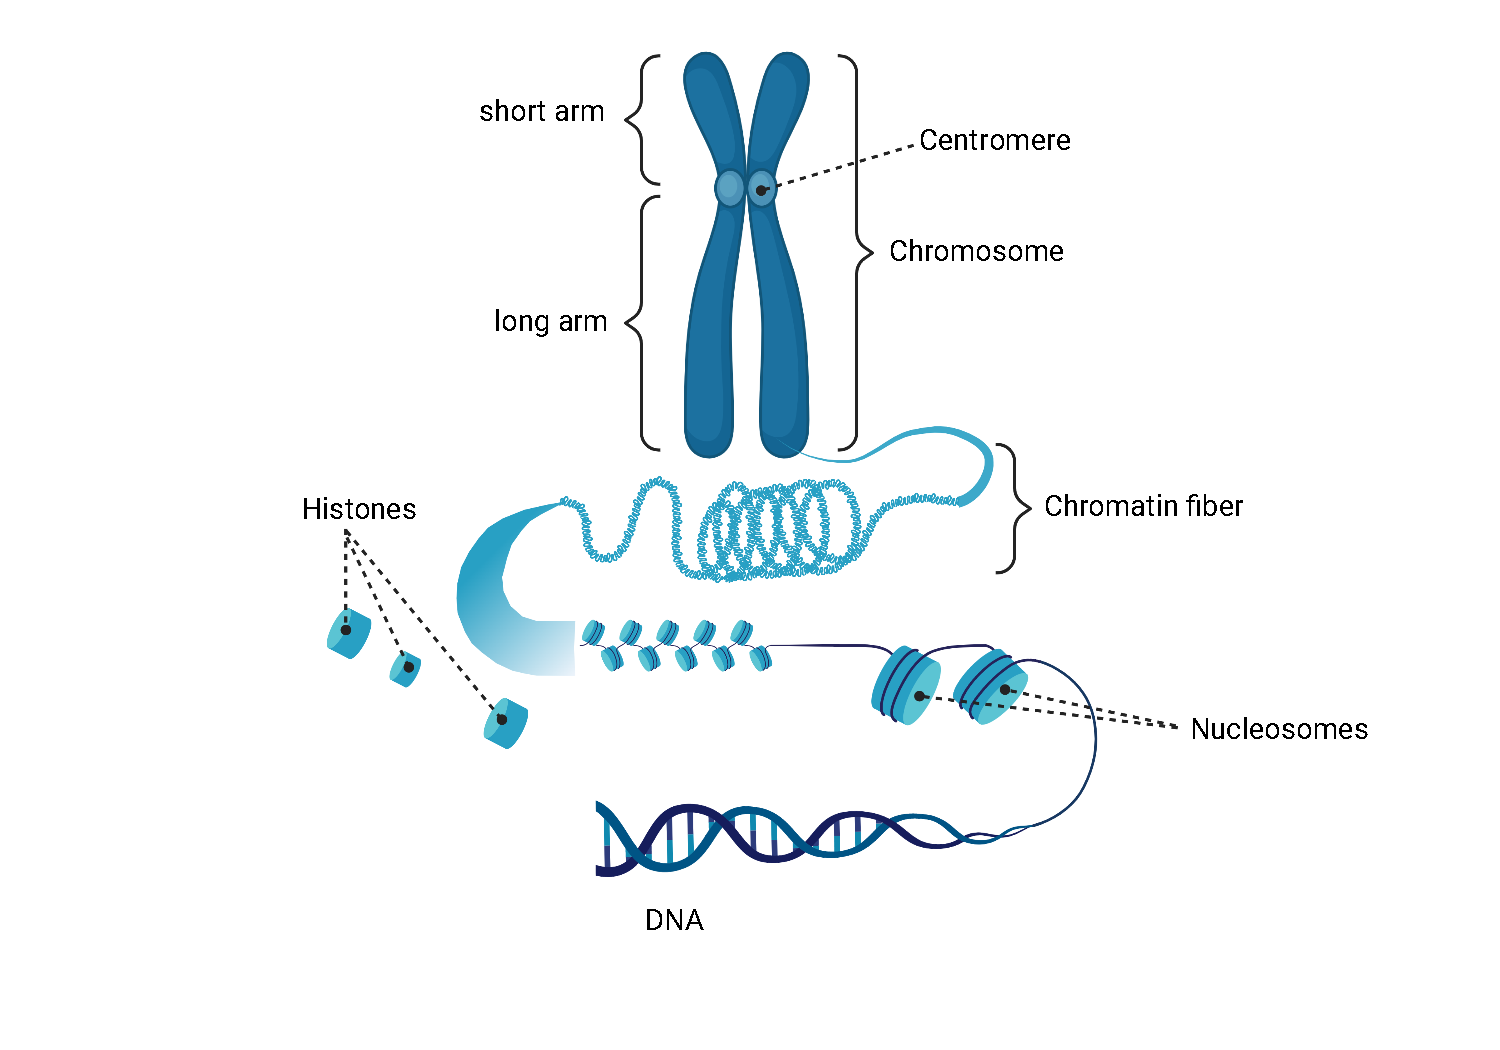
\includegraphics[width=0.9\linewidth]{Figures/ChromosomeStructure}
\caption[Overview Chromosome structure]{Structural overview of the metaphase condensed chromosome: DNA is first wrapped around Histones to form nucleosome, which then associate with each other to form the chromatin fiber, which in the metaphase of the cell cycle is condensed even more into the X-shaped chromosome}\label{fig:chromsomestructure}
\end{figure}

The DNA in eukaryotes however is not free floating around in the nucleus of a cell, but rather in most eukrayotic organisms, it is highly condensed and structured, first wrapped around nucleosomes like thread on a spool, then organised around histones, into either open (accessible) or closed chromatin, which then can be even further condensed into chromosomes, which have a X-like shape, with two shorter and two longer arms (\autoref{fig:chromsomestructure}). This allows some of the DNA to be accessible where the use of other areas can be restricted\cite{Hammond2017}. Through this restriction, the availability of certain genes, which are the sections of the DNA, which encode for short term storage molecules like RNA. This restriction plays an important role in cell fate and cell viability. Ultimately all information stored to create a new highly complex organism is stored in just the DNA of one cell. Whichever parts are used and how they are used decides the function and the identity of the cell\cite{Bonev2016}. 



\subsection[Ploidy]{Ploidy - its good to have a backup, if you do it right}
\label{intro-sec:ploidy}
Similar to the already discussed RAID-like setup of the DNA in two strands, another concept of data security, a spatial different storage is also implemented. Most eukaryotic organisms have at least two of each chromosome (diploid) with some species reaching up to septaploid\cite{Tateoka1975}. However, this concept is not the only reason for the ploidy of somatic cells. For sexually reproducing organisms, at least a diploid set of chromosomes is necessary to enable information to be joined from both parents. Germline cells (sperm and egg) are generally monoploid, such that the resulting cell will be diploid, but the ploidy of the somatic cells is not as uniform within a species, where it can vary between organisms based on gender or rank \cite{Trivers1976}. 
In most organisms, a change in ploidy is fatal \cite{Otto2007} and only partial ploidy changes like extra copies of chromosome 17 \cite{Gottlieb1962}, chromosome 18 \cite{Cereda2012} and chromosome 21 \cite{Hulten2008} are tolerated. These syndroms can occur when the is an uneven split of chromosomes during cell division.
The additional advantage, apart from sexual reproduction, is that a second almost identical copy of a chromosome allows repair of DNA, even when both strands are damaged, for example in a double strand break.
In this case, the information from the sister chromosome will be used, by first cutting the double strand break ends to have overhang (resection). This overhang will then merge with the sister chromosome's mirrored strand. In this state, the two chromosomes are fused together in a Holliday junction, which allows the missing part from the resection and the double strand break to be synthesised \cite{Lilley2000}. During this process, which is part of the homology directed repair (HDR) machinery, the sister chromosomes exchange parts of their DNA, when resolving the Holliday junction. As these stretches of DNA do not need to be 100\% identical, this plays and important role in evolution and diversity \cite{Hanage2006,Kong2013}.

\begin{figure}[!ht]
\centering
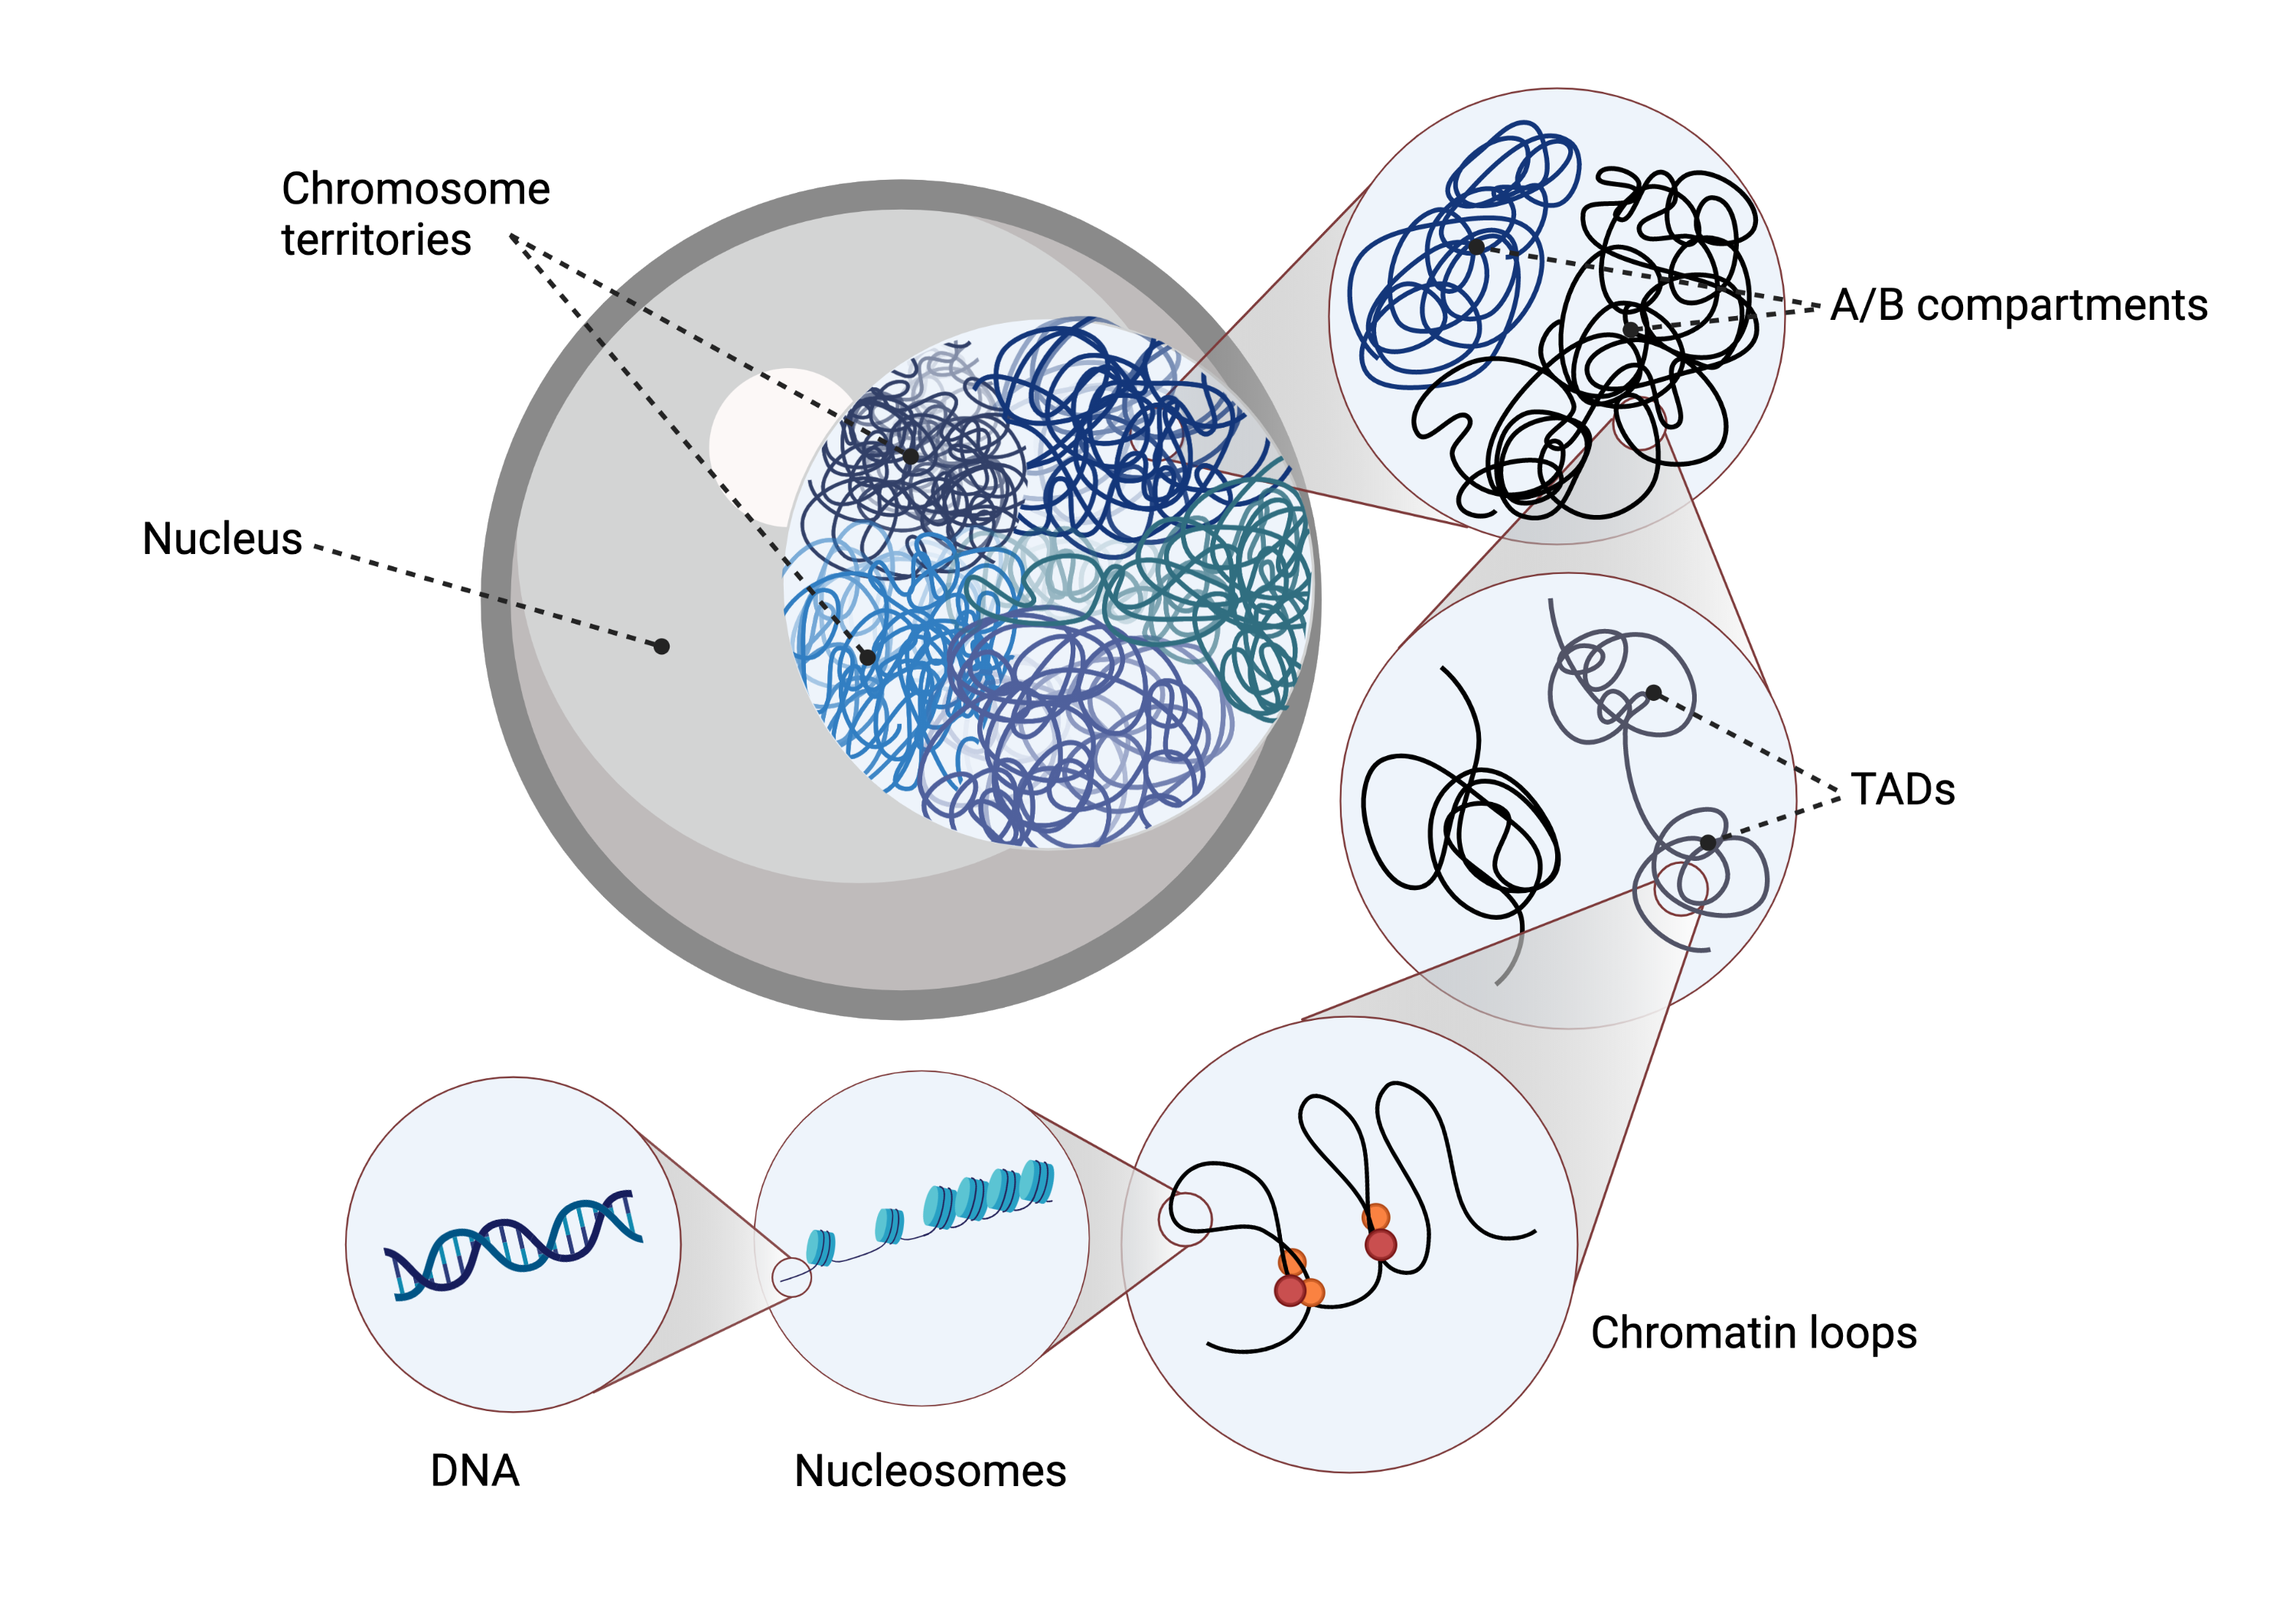
\includegraphics[width=0.9\linewidth]{Figures/ChromosomeTerritories}
\caption[Overview DNA structure]{Individual chromosomes occupy a subspace in the nucleus called chromosome territories. Chromosome territories can be further partitioned to distinct A and B compartments, which are enriched for active and repressed chromatin, respectively. Genomic regions within topologically associating domains (TADs) display increased interactions, while their interactions with neighbouring regions outside of the TADs are rather limited.}\label{fig:chromosometerretories}
\end{figure}

Even though this X-like structure is the most commonly used and known structure, the DNAs 3D structure is usually very different and only takes this shape for the very short time of the cell cycle. Most of the time, the chromosomes are unravelled into something resembling a ball of yarn, where the ``open`` chromatin regions are on the outside and the ``closed`` regions are ``hidden`` in the inside and each chromosome establishes its own ``territory`` inside the nucleus (\autoref{fig:chromosometerretories}). This structure allows another DNA cross over with non-sister chromsomes, which is called a chiasma.

\subsection[Mutations]{Phantastical mutations and where to find them}
\label{intro-sec:mutations}
However even though the DNA is highly stable and error correction methods are constantly working to not introduce any changes in the DNA, the source of evolution and adaptation of species is sourced in a steady mutation rate \cite{Darwin2010,Sprouffske2018}. These changes in normal tissue are mostly irrelevant to the organism as a whole and will not be passed on to the next generation. These changes are known as somatic mutations. This type of mutation accumulates in a cell linearly over the course of the lifespan of the cell and is not bound to just cell divisions\cite{Alexandrov2015,Moore2021}. 
In contrast, if one of those mutations occurs in the germline cell, eg. sperm or egg producing cells, these mutations will be propagated to all offspring and be present in all cells of that organism and in term all its offspring. These mutations are called germline mutations. These mutations are also called germline variants, as they establish in the population and represent a variation of the organism.
Mutations can also be classified depending on either their size ranging from single nucleotide polymorphisms (SNPs) over small insertions or deletions (InDels) to large structural changes, like the deletion of parts of or even a whole chromosome arm. like previously described with ploidy changes, usually smaller changes have less impact on the overall fitness of the organism, however even SNPs can lead to changes which are not compatible with life\cite{Shamseldin2015,Frey2021}.

